
\documentclass[11pt]{article}
\title{\textbf{Algorithmique Avancée}\\Projet London}
\author{Guillaume Magniadas}
\date{}
\usepackage{graphicx}
\usepackage{listings}
\usepackage[frenchb]{babel}
\begin{document}

\maketitle
\begin{figure}[htp]
\centering
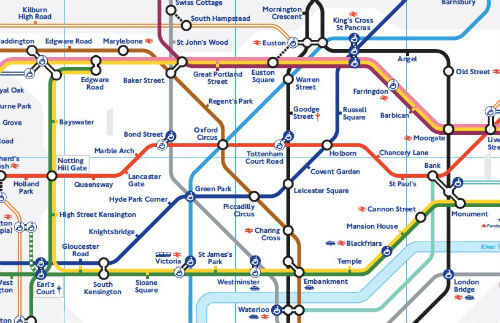
\includegraphics[scale=0.75]{plan-metro-londres-centre.jpg}
\caption{Métro de Londres}

\label{}
\end{figure}

\newpage
\tableofcontents
\newpage

	\section{Introduction}
	\subsection{Projet}
Ce projet consiste à représenter les structures de métro de Londres sous forme de graphe stocké dans deux structures différentes : Tableau de brin et matrice Compacte. Il faudra résoudre le problème du plus court chemin dans ces deux structures.
	\subsection{Objectifs}
Pour mener à bien ce projet, il y a plusieurs objectifs à atteindre :\\1: Stocker les données concernant les métros de Londres dans un fichier pour ensuite s'en servir pour remplir nos structures de graphe.\\2: Créer les structures de données qui accueilleront le graphe (Brin et matrice Compacte) ainsi qu'un lot de fonctionnalité pour utiliser ces dernières (fonction d'initialisation, de remplissage à partir d'un fichier, de libération de mémoire...)\\3: Créer une implémentation de l'algorithme de Dijkstra pour chacune de ces deux structures.


	\section {Données des Métro}
	\subsection{Récupérer les données}
Pour récupérer les données des lignes de Métro de Londres, plusieurs solutions s'offrent à nous. Trouver une liste déjà prête en ligne, à adapter pour qu'elle se prête bien à la création du graphe, ou alors réécrire la liste entière des métros de Londres et leur arrête. J'ai choisi la seconde option, je n'ai pas trouvé de liste qui me convenait en ligne.
\subsection{Organiser les données}
Pour simplifier la lecture du fichier par notre programme, avoir un fichier de données bien ordonnée est primordiale. J'ai décidé d'avoir une structure très simple pour ce fichier, la première ligne contiendra plusieurs informations sur les données à suivre : \\- le nombre de noeud\\- le nombre d'arêtes\\- le nombre de lignes de métro\\- le nombre de lignes dans le fichier concernant les lignes de métro\\
à noter que cette dernière donnée est importante car il est possible d'avoir des métros qui se découpe en plusieurs branches, et pour simplifier ces données, on coupe la saisie de ces lignes de métro en plusieurs lignes dans le fichier, une pour chaque branche. Donc le nombre de lignes concernant les lignes de métro peut être supérieur au nombre de lignes de métro.\\ \\
Voici un exemple de fichier compatible :

		\begin{lstlisting}
7 6 2 3
0 Brixton
1 Stockwell
2 Vauxhall
3 Pimlico
4 Victoria
5 Green_Park
6 Oxford_Circus
0 5 0 1 2 3 4 Victoria
1 3 3 4 5 Circle
1 3 3 5 6 Circle

\end{lstlisting}

La première ligne indique qu'il y a 7 stations de métro, 8 arêtes, 2 lignes de métro (Victoria et Circle) et qu'il y a 3 lignes dans le fichier concernant les lignes de métro.\\
Les 7 lignes qui suivent sont les stations de métro avec leurs identifiants et leur nom respectif\\
Les 3 dernières lignes sont les informations sur les lignes de métro.
Il y a la ligne Victoria qui a pour identifiant 0 et possède 5 stations, allant de Brixton à Victoria.
Il y a la ligne Circle qui elle est coupée en deux lignes dans le fichier.

\section{Création des structures de données}
Chacune des deux structures de données (Brins et matrice Compacte) sont différentes mais reste des structures classiques et possèderont des fonctionnalités similaires telles qu'une fonction pour les initialiser, les remplir et les libérer.\newline
Note : Nous parlerons aussi de la structure d'arbre de recherche de mots.
\subsection{Brins}
Toutes les fonctionnalités concernant la structure tableau de brins se trouvent dans les fichiers graph.h et graph.c.
Pour représenter un graphe avec un tableau de brin, j'ai créé plusieurs structures.

\subsubsection{Graph}
		\begin{lstlisting}
struct Graph{

	Vertice* vertices;
	unsigned int nbVertice;

	Strand* strands;
	unsigned int nbStrand;


	char** idToLinesName;
	unsigned int nbLine;

};

\end{lstlisting}
Elle est composée d'un tableau de Noeud, d'un tableau de Brins et d'un tableau de String pour stocker les noms des lignes.\\
\subsubsection{Vertice}
\begin{lstlisting}
struct Vertice{ // Sommet
	int firstStrand;

	char* label;
};
\end{lstlisting}

Elle contient un entier firstStrand qui contiendra l'index du premier brin attaché à ce noeud et un string qui contiendra le nom de la station de métro de ce noeud.\\
\subsubsection{Strand}
\begin{lstlisting}
struct Strand{ //Brin
	unsigned int vertice;
	int nextStrand;
	
	//If it's neg or pos
	int type;

	unsigned int lineId;

};
\end{lstlisting}
Elle contient l'index du noeud auquel le brin est attaché, l'index du prochain brin de ce noeud, un type, qui permet de savoir si on doit retirer 1 ou ajouter 1 à l'index de ce brin pour récupérer sa paire et l'identifiant de la ligne de métro de ce brin.\\
La variable type vous choque peut-être, dans un tableau de brin classique, un brin d'index n à pour paire le brin d'index -n. Les index d'un tableau ne pouvant certainement pas être négatifs, j'ai trouvé cela plus intéressant de quand même stocker tous les brins dans un même tableau avec chaque paire possédant un index voisin entre elles. Cela permet de garder un accès en temps constant au brin pair et de ne garder qu'un seul tableau de brin. Il faut en contrepartie savoir s'il s'agit du voisin d'index + 1 ou - 1, c'est cela que l'on stocke dans type.\\
\subsection{Matrice Compacte}
Toutes les fonctionnalités concernant la structure de matrice compacte se trouvent dans les fichiers mcoGraph.h et mcoGraph.c.
Pour représenter cette structure de données, j'ai créé une structure.
\subsubsection{Matrix}
\begin{lstlisting}
struct Matrix{

	char **stationName;

	char **lineName;
	unsigned int nbLine;

	int *data;

	unsigned int size;
	unsigned int width;

};
\end{lstlisting}
Elle est composée d'un tableau d'entier data pour stocker toutes les arêtes entre les noeuds (qui seront donc les arêtes entre les noeuds d'index x et d'index y), de size et width, qui stockeront la taille de la matrice et sa longueur. Il y a aussi deux tableaux de string, un qui stocke le nom des lignes de métro et un qui stocke le nom des stations de métro.\\
\subsection{Arbre de recherche de mots}
Pour ce projet, il est aussi important d'avoir une interface utilisateur simple permettant de sélectionner les stations par leur nom. Et pour garder un tout cohérent et performant, plusieurs choix s'offrent à nous. Une hashmap aurait pu être une bonne solution mais si on veut offrir la meilleure expérience utilisateur possible, il faut aussi permettre l'auto complétion des mots, pour terminer les noms de stations écrits par l'utilisateur. Et pour cela, j'ai choisi de faire un arbre de mots.\\
Cette structure d'arbre possède plusieurs fonctionnalités, des fonctions pour ajouter des mots, pour voir si un mot existe, compléter la fin d'un mot.\\
Elle possède des fonctions de re-réservation de mémoire dynamique pour ne jamais être limité par la taille.\\
Cet arbre est composé de deux structures principales :
\subsubsection{SearchingTree}
\begin{lstlisting}
struct SearchingTree {

	int* charToIndex;
	int charToIndexReserved;

	TreeNode** nextNodes;
	int nextNodesSize;
	int nextNodesReserved;

};
\end{lstlisting}
Il s'agit de la structure principale de l'arbre. Elle contient un tableau d'entier qui permet de récupérer la position de l'arbre qui fait suite à ce caractère dans nextNode, qui est donc un tableau de noeud, une structure dont nous allons parler juste en dessous. Elle contient aussi des variables de taille, la taille du tableau de caractère réserve, pareil pour le tableau de noeud mais avec une subtilité supplémentaire, on différencie sa taille et la taille réservée. Cela permet d'avoir un vecteur dynamique, dans lequel on peut continuer d'insérer en sa fin des valeur tant que la taille est inférieure à la taille réservée.\\
\subsubsection{TreeNode}
\begin{lstlisting}
struct TreeNode {

	unsigned int value;

	char c;
	int end;

	SearchingTree* nextTree;

};
\end{lstlisting}
Cette structure représente les noeuds de l'arbre. Elle contient le caractère représenté par ce noeud, si le caractère marque une fin de mot, et un pointeur sur la suite de l'arbre. Ce pointeur est potentiellement nul s'il n'y a pas de suite après cette lettre.\\
\subsection{Autre}
Certaines structures utiles ont été créé. Parmi celles-ci il y a sortedQuintupletList (dans les fichiers sortedQuintupletList.c et .h) et sortedTupleList (dans les fichiers sortedTupleList.c et .h) qui sont des listes triées contenant respectivement 5 et 3 entiers par pointeur de la liste.
Il y a aussi les structures BrandPath et NodePath qui servent à stocker le chemin retourné par l'algorithme de Dijkstra (un via les brins parcourus et l'autre par les noeuds parcouru).\\
\section{Algorithme de Dijkstra} 

Ce projet contient 2 implémentations de l'algorithme de Dijkstra. Une pour la structure de brins, une pour la matrice compacte. Le principe de l'algorithme en demeure quand même le même. Je vais expliquer les plus gros points de cet algorithme pour la structure à brin et je passerais sur les petites subtilités de la version pour la structure matrice compacte.
\subsection{Dijkstra pour Brins}
\begin{lstlisting}
int* visitedStrand;
TupleNode* tempoTuple;
\end{lstlisting}\\
Pour commencer, on peut remarquer que la fonction utilise un tableau d'entier et une structure TupleNode. Ce tableau d'entier permet de savoir si un brin a déjà été visité, si oui si il est fini ou s'il n'est pas fini, son meilleur cout. Chaque index correspond à un brin, la valeur 0 veut dire non exploré, inférieur à 0 veut dire terminé (et on stocke le brin qui a mené à ce brin en stockant son index négatif moins 1) et supérieur à 0 veut dire déjà visité mais pas terminé, et la valeur est le cout du meilleur passage.\\
La structure tempoTuple est une liste chainée stockant 3 valeurs. Elle est aussi automatiquement triée à chaque ajout de valeur, se basant sur la première des 3 valeurs et du plus petit au plus grand. Cette liste nous permettra de stocker les meilleurs brins, on stocke donc leur cout, leur index et le brin qui nous a menés à lui.\\
La sauvegarde des anciens brins sert surtout à la fin de l'algorithme à retracer le chemin qui a mené au plus court chemin.\\
\begin{lstlisting}
BrandPath* pathToReturn;
\end{lstlisting}
On déclare aussi ce pointeur qui servira à accueillir le chemin de brin final.\\
\begin{lstlisting}
    do{
        [...]
    while(actualStrandIndex != -1);
\end{lstlisting}\\
La boucle principale est une boucle infinie qui break quand le meilleur brin actuel est un brin attaché au noeud final. S'ensuit la boucle juste en dessous, un do while. Cette boucle part du brin actuel (le brin actuel est le brin gagnant d'un tour de l'algorithme, au début de l'algorithme il est le premier brin du noeud de départ) et avance dans tous les brins suivants (nextStrand dans la structure brin) jusqu'à ce que le prochain brin soit l'index -1 qui signifie qu'on a parcouru tous les brins du noeud.
Dans le do, on vérifie si le brin sur lequel on est n'est pas fini dans le tableau visitedStrand, s'il a deja été visité mais que son nouveau cout est plus petit que son ancien ou qu'il n'a pas encore été visité, on l'ajout à la liste costAndStrand.\\
\begin{lstlisting}
do{

    tempoTuple = getFirstList(&costAndStrand);
    
    actualStrandIndex 		= tempoTuple->second;
    actualCost                  = tempoTuple->first;
    oldWinnerStrandIndex 	= tempoTuple->third;
    
    deleteFirstList(&costAndStrand);

}
while(visitedStrand[actualStrandIndex] < 0);
\end{lstlisting}\\
Nous avons ensuite un nouveau do while, il récupère le premier élément de la liste costAndStrand et le supprime (le premier element est donc le brin au cout le plus bas) et cela tant que le brin récupéré n'est pas fini. Pourquoi un brin pourrait être fini dans cette liste alors qu'on n'insère un élément que s'il n'est pas fini ? Car il est possible qu'entre-temps l'on trouve un chemin moins couteux jusqu'à ce brin et par conséquent qu'on ait déjà sélectionné ce brin auparavant mais vu qu'a l'insertion de brin dans la liste, on n'enlève pas l'ancien meilleur cout, il reste des résidus, d'où cette vérification. J'ai préféré rajouter cette simple vérification plutôt qu'enlever les anciens meilleur brin de la liste, ce qui serait couteux car forcerait un parcours de cette dernière.\newline
\\
Une fois cette dernière boucle faite, on remplace le brin actuel par le brin sélectionné dans la liste, et s'il n'est pas attaché au noeud d'arrivée, on recommence.\\


\begin{lstlisting}
visitedStrand[actualStrandIndex] = -1*(oldWinnerStrandIndex+1);
visitedStrand[actualStrandIndex + actualStrand->type] =
-1*(oldWinnerStrandIndex+1);
\end{lstlisting}

Ces lignes sauvegardes le brin qui a mené au brin actuel dans le tableau visitedStrand (on sauvegarde aussi dans la paire du brin pour bien le marquer comme fini).\\
Voilà pour le coeur de l'algorithme.\\
Après celui-ci, quelques lignes sont consacrées au remplissage du BrandPath (pathToReturn). C'est un simple parcours en arrière du tableau visitedStrand. Ce code est assez simple donc je ne passerais pas dessus.\\
\subsection{Dijkstra pour Matrice Compacte}
Comme dit précédemment, l'algorithme est très similaire mais il y a quand même quelques subtilités à noter.

\begin{lstlisting}
    CostAndDone* saved;
    QuintupletNode* tempoQuintuplet;
\end{lstlisting}
Le tableau d'entier précédent est remplacé par un tableau de CostAndDone qui est une structure qui contient 2 tableaux, un d'entier donePerLine et un d'entier non signé costPerLine. Vu que les noeuds ne permettent pas de stocker autant d'information que les brins, on doit pouvoir différencier un passage sur un noeud en venant d'une ligne A et d'une ligne B car un changement de ligne pourrait engendrer un cout supplémentaire, donc on doit prendre cela en compte. Ces deux tableaux dans CostAndDone sont initialisé à la taille 2 puissances "nombres de lignes de métro". Cela permet d'avoir un index pour chaque combinaison de lignes de métro.\\
La liste n'est plus une liste stockant 3 valeurs, mais une liste stockant 5 valeurs, le cout, le noeud, la ligne de métro, l'ancien noeud et l'ancienne ligne de métro. Pour les mêmes raisons que la structure précédente, nous avons besoin de stocker plus d'informations pour les noeuds, nous sauvegardons donc aussi la ligne et l'ancienne ligne.

\begin{lstlisting}
    for(i = 0; i < graph->width; ++i){
        [...]
    }
\end{lstlisting}
La boucle do while est ici remplacé par une boucle for plus classique pour parcourir la ligne du noeud courant (donc les arêtes entre le noeud courant et i).\\
Les premières lignes dans ce for sélectionnent l'arête, à noter que la structure matrice compacte a été optimisée, j'en reparlerais dans la section optimisation.\\

\begin{lstlisting}
    saved[actualNode].donePerLine[actualLineId] = 1 + oldNode;
    saved[actualNode].costPerLine[actualLineId] = oldLineId;
\end{lstlisting}
Comme pour le Dijkstra de la structure brins mais pour les noeuds, on sauvegarde le noeud qui a mené au noeud actuel et aussi la ligne qui a été utilisée.
\subsection{Affichage}
Il reste un détail, pour pouvoir utiliser les structures NodePath et BrandPath, des fonctions d'affichage son disponible, elles afficheront dans le terminal un chemin à suivre facilement compréhensible par un humain.
\section{Optimisation}
Une optimisation majeure a été faite pour la structure Matrice compacte.\\
La matrice compacte possède un défaut majeur, elle nous force à vérifier toutes la possibilité d'arêtes pour un noeud vers chaque noeud, car on ne sait pas si valeur de la ligne du noeud est vide ou non. Pour pallier ce problème, j'ai décidé de rajouter une valeur négative, qui serait l'index de la prochaine arête au négatif - 1. Du coup sur une ligne de la matrice, quand une valeur est 0, il suffit de sauter à l'index de ligne (valeur * -1) - 1, si la valeur est positive, il y a une arête et si la valeur est égale à 0, il n'y a plus d'arête. Cette optimisation améliore grandement les performances du parcours sur cette structure, bien qu'elle reste en moyenne 10 fois plus lente que pour la structure à brins sur ce graphe.\\
À noter que d'après quelques tests effectués, la structure matrice Compacte dépassait la structure à brins dans des graphes avec moins de noeud, (moins de 100).
\section{Notes}
Voilà pour la partie code, je tiens à préciser que le code est très commenté donc si quelque chose ne reste pas clair, vous devriez regarder le code, il y aura surement des commentaires pour répondre à votre question. (Ils sont en anglais)
\section{Utilisation}
Pour compiler le programme, lancez make :
\begin{lstlisting}
$ make
\end{lstlisting}
une fois compilé, vous n'avez plus qu'a le lancer :
\begin{lstlisting}
$ ./exe.out
\end{lstlisting}
Dans le programme, vous devez d'abord choisir 2 stations, pour vous aider dans votre choix, vous pouvez écrire le début des lettres d'une station et il vous proposera des complétions de votre début de mot.\\
Une fois les deux stations choisies, il vous demandera une option de parcours, le plus court chemin (0) ou le chemin avec le moins de correspondances (1).\\
Et enfin, il vous demandera quelle structure voulez-vous utiliser (brins 0, matrices compacte 1) ou si vous voulez comparer les deux en temps (2).
\section{Traces d'exécution}
Exemple d'une exécution classique pour récupérer un itinéraire :
\begin{figure}[htp]
\centering
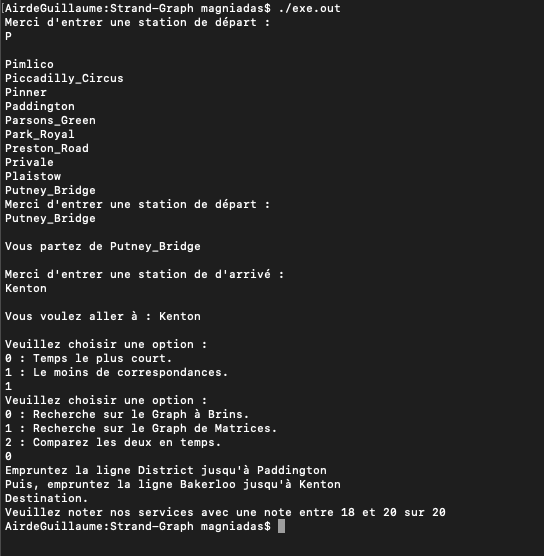
\includegraphics[scale=0.6]{Trace_1.png}
\caption{Exemple 1}
\label{}
\end{figure}
\newpage
Exemple d'une exécution où l'on compare les deux structures en temps :
\begin{figure}[htp]
\centering
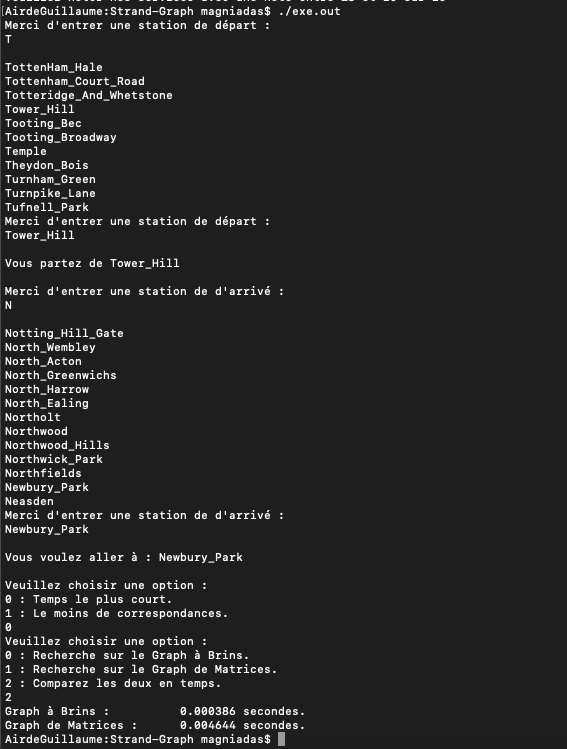
\includegraphics[scale=0.50]{Trace_2.png}
\caption{Exemple 2}
\label{}
\end{figure}
\end{document}




